\section{Use Case: Click \& Ride App and Netzfahrplan}
\label{chap:useCases}
In this section, we describe the use cases which were used to proof that our approach for the automatic opitimized creation of railway timetables performes. For this we set ourselves three goals: 

\begin{itemize}
	\item[1)] An customer's request suppose to be proceed after three minutes with the Click\&Ride App
	\item[2)] The Systemtrassen are suppose to increase the capacity of the german railway network
	\item[3)] With the Belegung on the Systemtrassen we minimize the time customer spend within the network
\end{itemize}

\subsection{Click \& Ride App}
\label{chap:CnR}
For a short-term train path request, e.g. a train run for the next day, we can improve the response time to the railway operator by using our approach in a fully automated process. We will introduce the new way of booking a train path with a mobile application called "Click\&Ride-App". We commit to get the railway operator a train path offering within no longer than three minutes. In comparison, today's process for manual planning takes several hours or even up to three days. To ensure a maximum duration of three minutes we need to automazie every single step in the plannning process. A simplified process sequence is shown in figure \ref{fig:process_sequence}. 
\begin{figure}[htb]
	\centering
	% If you include a JPG file, 
	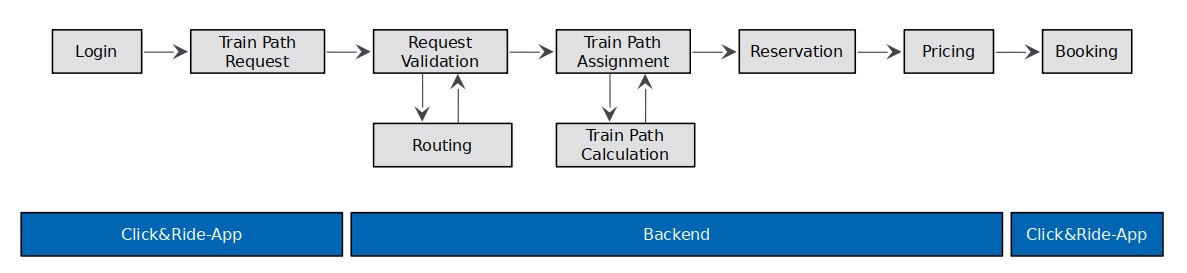
\includegraphics[width=\textwidth]{Bilder/process_sequence.jpg}
	% Else if you include an EPS file 
	%    (it may need an interpreter for the PostScript language, e.g. Ghostscript), 
	%\includegraphics[scale=0.30]{Fig1_Track.eps}
	\caption{Process of Click\&Ride}
	\label{fig:process_sequence}
\end{figure}

Click\&Ride is a new B2B channel so only railway operators may use the functionalities. After logging in, the the train path request will be submitted to the backend processes. At first there is a validation service that ensures formal and technical fit to the lines that will be used. For example an electric vehicle cannot use a line with no overhead line. If there are any problems with the train path request the railway operator gest instant feedback on the app's screen and can fix the problem.

\subsection{Netzfahrplan}
\label{chap:Netzfahrplan}
The new process of creating the Netzfahrplan will be devided into two steps. The first step is the manuall creation of the 
public transport which takes place during the day and the scound step is the automatic creation of the freight transport during the night. This interaction takes place every day during the period of the creation of the Netzfahrplan. As a consequence the manuall and the automatic generation can interact with each other every day. \\
\\
\textbf{\textcolor{red}{Falls noch Platz, könnte hier das Schaubild hinzufügen}}
%
\begin{table}[h]
	\centering
	\caption{Results for Netzfahrplan}
	\label{tab:result_Netzfpl}
	\begin{tabular}{lcccc} \hline
		\textbf{Text Style}   & \textbf{Font} & \textbf{Style} & \textbf{Size (pt)} \\ \hline
		Main text             & Times         & regular        & 10                 \\
		Section heading       & Times         & bold           & 12                 \\
		Subsection heading    & Times         & bold           & 10                 \\
		Subsubsection heading & Times         & bold           & 10                 \\ \hline
	\end{tabular}
\end{table}
\par


